
\documentclass[12pt,letterpaper]{IEEEtran}
\usepackage[utf8]{inputenc}
\usepackage[spanish]{babel}
\usepackage{geometry}
\geometry{left=25mm, right=25mm, top=30mm, bottom=35mm} 
\renewcommand{\baselinestretch}{1.5}
\usepackage{amsmath}
\usepackage{amssymb}
\usepackage{placeins}
\usepackage{graphicx}%%
\usepackage{mathrsfs}%para la transformada inversa
\usepackage{cancel}

\begin{document}
	\title{\sc{\textbf{Instituto Tecnologíco de Morelia}} \\ \sc\textbf{Control}}
	\date{24 de noviembre del 2017}
	\author{ \textbf{PRACTICA No.2 Polos y ceros encontrados por inspección} \\\textbf{ Departamento de Ingeniería Electrónica} \\\textbf{Profesor} \\Gerardo Marx Chávez Campos \\ \textbf{Alumnos}  \\ Hernandez Arteaga Aracely Lizeth 14121092 \\ Erick David Bedolla García 14121081}
	\maketitle
	\section{Introducción}
	
	En la práctica anterior de este curso se analizo un sistema de control en el cual encontrabamos un modelo matematico del sistema, una vez obtenido en modelo se puede observar su comportamiendo mediante varios metodos.
	\\
	Los polos y los ceros permiten la caracterización dinámica de un sistema en este caso el método utilizado fue el método de inspección.
	\\
	En el análisis y diseño de sistemas de control, se debe tener una base de comparación del
	comportamiento de diversos sistemas de control. Esta base se configura especificando las señales
	de entrada de prueba particulares y comparando las respuestas de varios sistemas a estas señales
	de entrada.
	Muchos criterios de diseño se basan en tales señales o en la respuesta del sistema a los cambios
	en las condiciones iniciales (sin señales de prueba). El uso de señales de prueba se justifica
	porque existe una correlación entre las características de respuesta de un sistema para una señal
	de entrada de pru
	eba común y la capacidad del sistema de manejar las señales de entrada reales. 
	\\Señales de prueba típicas. Las señales de prueba que se usan regularmente son funciones
	escalón, rampa, parábola, impulso, etc. Con estas señales de prueba, es posible realizar con
	facilidad análisis matemáticos y experimentales de sistemas de control, ya que las señales son funciones del tiempo muy simples.
	\\\\La forma de la entrada a la que el sistema estará sujeto con mayor frecuencia en una operación
	normal determina cuál de las señales de entrada típicas se debe usar para analizar las características
	del sistema. Si las entradas para un sistema de control son funciones del tiempo que
	cambian en forma gradual, una función rampa será una buena señal de prueba. Asimismo, si un
	sistema está sujeto a perturbaciones repentinas, una función escalón será una buena señal de prueba;
	y para un sistema sujeto a entradas de choque, una función impulso será la mejor. Una vez
	diseñado un sistema de control con base en las señales de prueba, por lo general el comportamiento
	del sistema en respuesta a las entradas reales es satisfactorio. El uso de tales señales de prueba
	permite comparar el comportamiento de todos los sistemas sobre la misma base.
	\\ Para obtener estos modelos matematicos usamos el método de inspección el cual consiste en encontrar los polos y los ceros de un sistema en este caso un sistema RL el cual se muestra en la siguiente figura.
	
	\begin{figure}[h!]
		\centering
		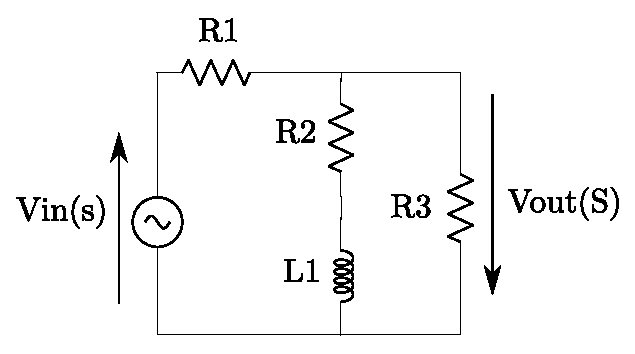
\includegraphics[width=0.7\linewidth]{Circuito}
		\caption{Circuito RL }
		\label{fig:circuito}
	\end{figure}
	
	\section{Metodología}
	\subsection{Analisis por inspeccion}
	\textbf{Ganancia en CD ($G_{0}$) por inspección}\\
	
	
	Primeramente buscaremos la ganancia en CD($G_{0}$) para lo cual se cortocicuitara el inductor, esto debido a que ya se conoce que en CD el inductor tiene un comportamiento  como el de un cable a manera que nuestro circuito quedara de la siguiente manera:
	
	\begin{figure}[h!]
		\centering
		\includegraphics[width=0.7\linewidth]{Circuito2}
		\caption{Circuito RL con L cortocircuitada}
		\label{fig:circuito2}
	\end{figure}
	
	ahora bien podemos analizar nuestro circuito de la siguiente manera:
	
	$$V_{out}(s)=V_{in}(s)\frac{R2\parallel R3}{R1+R2\parallel R3}$$\\
	Desarrollando las operaciones podemos obtener el siguiente resultado:
	$$\frac{V_{out}(s)}{V_{in}(s)}=\frac{\frac{R2 R3}{R2+R3}}{R1+\frac{R2 R3}{R2+R3}}$$
	
	$$\frac{V_{out}(s)}{V_{in}(s)}=\frac{\frac{R2 R3}{\cancel{R2+R3}}}{\frac{R1R2+R1R3+R2 R3}{\cancel{R2+R3}}}$$
	
	
	
	$$\frac{V_{out}(s)}{V_{in}(s)}=\frac{R2R3}{R1R2+R1R3+R2R3}=G_0$$
	
	
	
	\textbf{Obtencion de los Ceros ($\omega_{z1}$)}\\
	Ahora se realizara el analisis de la rama que tiene el inductor ya que es el unico elemento en nuestro circuito que puede causar ceros debido a su reaccion con la frecuencia.\\
	De manera que obtenemos lo siguiente igualando a cero :\\
	
	$$R2+SL=0$$
	
	
	Ahora se divide todo entre R2:
	
	$$1+\frac{SL}{R2}=0$$
	
	Sabiendo que la exprecion general es:
	
	$$\frac{S}{\omega _{z1}}=\frac{SL}{R2} $$
	
	Obtenemos que $$\omega _{z1}=\frac{R2}{L}$$
	
	\textbf{Obtencion de los Polos ($\omega_{p1}$)}\\
	Para encontrar los polos de nuestro cistema se n¡ecesita cortocircuitar la fuente ademas de quitar el inductor para que nuestro circuito quede de la siguiente manera:\\
	
	\begin{figure}[h!]
		\centering
		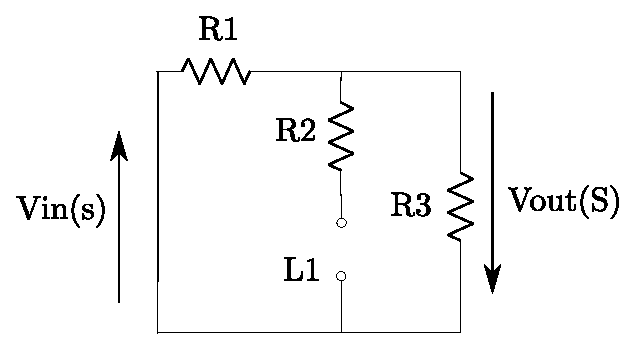
\includegraphics[width=0.7\linewidth]{Circuito3}
		\caption{Circuito RL}
		\label{fig:circuito3}
	\end{figure}
	
	
	
	obteniendo una resistencia equivalente de 
	
	$$R_{eq}=R2+(R1\parallel R3)$$
	
	ahora bien se tiene que:
	
	$$\omega_{p1}=\frac{1}{\tau}=\frac{R_{eq}}{L}$$
	
	Reescribiendolo tenemos:
	
	$$\omega_{p1}=\frac{R2+(R1\parallel R3)}{L}$$
	
	$$\omega_{p1}=\frac{\frac{R2R1+R2R3+R1R3}{R1+R3}}{L}$$
	
	$$\omega_{p1}=\frac{R2R1+R2R3+R1R3}{L(R1+R3)}$$
	
	Finalmente nuestra funcion de transferencia quedaria de la siguiente manera:
	
	$$H(s)=\frac{R2\parallel R3}{R1+(R2\parallel R3)}\frac{1+\frac{SL}{R2}}{1+\frac{SL}{R2+(R1\parallel R3)}}$$  
	
	\subsection{\textbf{Analisis algebraico para encontrar ganancia en CD, polos y ceros }}
	
	Primeramente se busco reducir el circuito y asi encontrar un $Z_{eq}$
	
	De manera que obtenemos:
	
	$$Z_{eq}=(R2+SL)\parallel R3$$
	
	$$Z_{eq}=\frac{(R2+SL)(R3)}{R2+SL+R3} $$ 
	
	$$Z_{eq2}=\frac{R2R3+SLR3}{R2+SL+R3}$$
	
	Aplicando un divisor de tencion podemos obtener el voltaje de salida 
	
	$$V_{out}=V_{in}\frac{\frac{R2R3+SLR3}{R2+SL+R3}}{R1+\frac{R2R3+SLR3}{R2+SL+R3}}$$
	
	una vez que tenemos esto podemos relacionar el voltaje de salida y el de entrada  asi:
	
	$$\frac{V_{out}}{V_{in}}=\frac{\frac{R2R3+SLR3}{R2+SL+R3}}{R1+\frac{R2R3+SLR3}{R2+SL+R3}}$$
	
	$$\frac{V_{out}}{V_{in}}=\frac{\frac{R2R3+SLR3}{R2+SL+R3}}{\frac{R2R3+SLR3+(R1)(R2+SL+R3)}{R2+SL+R3}}$$
	
	$$\frac{V_{out}}{V_{in}}=\frac{R2R3+SLR3}{R2R3+SLR3+R1R2+R1SL+R1R3}$$
	
	Esta se podria considerar ya la funcion de transferencia mas sin embargo no se encuentra de manera que podamos identificar si por inspeccion o de manera algebraica se obtienen los mismos resultados, asi que procedemos a desarrollarla de la siguiente manera:\\
	
	$$\frac{V_{out}}{V_{in}}=\frac{R2R3(\frac{SL}{R2}+1)}{R2R3(1+\frac{SL(R1+R3)}{R1(R2+R3)+R2R3})+R1(R2+R3)}$$
	
	$$\frac{V_{out}}{V_{in}}=\frac{R2R3}{R2+R3(R1+\frac{R2R3}{R2+R3})} \frac{\frac{SL}{R2}+1}{1+\frac{SL(R1+R3)}{R1(R2+R3)+R2R3}}$$
	
	$$\frac{V_{out}}{V_{in}}=\frac{R2\parallel R3}{R1+(R2\parallel R3)} \frac{\frac{SL}{R2}+1}{1+\frac{SL(R1+R3)}{R1(R2+R3)+R2R3}}$$
	
	$$\frac{V_{out}}{V_{in}}=\frac{R2\parallel R3}{R1+(R2\parallel R3)} \frac{\frac{SL}{R2}+1}{1+\frac{SL(R1+R3)}{R1R3+R2(R1+R3)}}$$
	
	
	$$\frac{V_{out}}{V_{in}}=\frac{R2\parallel R3}{R1+(R2\parallel R3)} \frac{\frac{SL}{R2}+1}{1+\frac{SL(R1+R3)}{R1+R3\frac{R1R3}{R1+R3}+R2}}$$\\
	
	Forma general:
	
	$$\frac{V_{out}}{V_{in}}=\frac{R2\parallel R3}{R1+(R2\parallel R3)} \frac{\frac{SL}{R2}+1}{1+\frac{SL}{R1\parallel R3+R2}}=H_(s)$$
	
	\subsection{\textbf{Respuesta en Scilab.}}
	
	
	
	\subsection{\textbf{Programación en LTspice.}}
	
	Para simular el circuito RL en LTspice, utilizamos los siguientes códigos:
	\\
	;Circircuto RL\\
	Vin 1 0 AC 2.5\\
	R1 1 2 10k\\
	R2 2 3 3.9k\\
	R3 2 0 10k\\
	L1 3 0 4.29mH\\
	.ac dec 10 10Hz 1000000k\\
	.end\\
	
	
	La programacion en  LTspice concistio basicamente en saber ubicar los nodos y elementos que estaban conectados a ellos de manera que se le dieron valores y logramos ver las respuestas que tendrian.
	
	\subsection{\textbf{Calculos de $\tau$}}
	
	Para calcular $\tau$ del circuito RL tenemos que:
	
	$$\tau=\frac{L}{R_eq}$$
	
	Tenemos los datos de:\\
	L=4.29mH \\
	$R_eq=(R_1||R_3)+R_2$\\
	Por lo tanto, tenemos que:
	
	$$\tau=\frac{4.29mH}{8.9k}=482.0n S$$
	
	
	Para calcular $\tau$ del circuito RC tenemos que:
	
	$$\tau=C*R_eq$$
	
	
	Como sabemos:
	
	$C=1\mu F$ y $R_eq=8.9k$
	
	Por lo tanto, tenemos que:
	
	$$\tau=8.7mS$$
	
	\subsection{\textbf{Simulacion en LTspice:}}
	\begin{center}
		A continuacion podemos ver las simulaciones realizadas en LTspice la cual es la respuesta en el tiempo de una funcion escalon para nuestro circuito RL y la respuesta en frecuencia.\\
		
		\includegraphics[width=0.8\linewidth]{escalon}
		
	\end{center}
	\begin{center}
		
		\includegraphics[width=0.8\linewidth]{frecuenciaRL}
		
	\end{center}
	
	
	\subsubsection{\textbf{Barrido en frecuencia}}
	Se usaron cursores para medir el voltaje maximo de ahi se multiplicopor .63 para obtener el $\tau$ medido
	\begin{center}
		
		\includegraphics[width=0.8\linewidth]{resp}
		
	\end{center}
	
	\begin{center}
		
		\includegraphics[width=0.8\linewidth]{rd}
		
	\end{center}
	\begin{center}
		
		\includegraphics[width=0.8\linewidth]{de}
		
	\end{center}
	
	
	\section{\textbf{Conclusiones:}}
	\textbf{Hernandez Arteaga Aracely Lizeth 14121092}\\
	esta practica realmente me ayudo a reforzar lo visto en clase ya que se usaron dos metodos para lograr encontrar la funcion de transferencia, por mi parte considero el metodo de ispeccion es mas sensillo de llevar acabo.\\
	Como pudimos notar hay cierta diferencia entre lo medido y lo simulado esto debido a que inductor usado no es para altas frecuencias.\\
	Para terminar se podria decir que hay factores que pudieran alterar los resultados ya al momento de realizar las cosas fisicamente y que teoricamente no se perciben.  
	
	\textbf{Erick David Bedolla García 14121081}
	
	En esta práctica se tuvo la oportunidad de utilizar otro método para encontrar la función de transferencia de un sistema. Otra de las cosas interesantes fue implementar el modelo obtenido y ver como difieren los resultados teoricos de los prácticos. Otra cosa a mencionar es que se pudo observar como los sistemas estan limitados por sus componentes, ya sea porque no pueden trabajar a altas frecuecias o temperaturas las cuales pueden afectar al sistema y hacerlo inestable.












































\end{document}